%%%%%%%%%%%%%%%%%%%% author.tex %%%%%%%%%%%%%%%%%%%%%%%%%%%%%%%%%%%
%
% sample root file for your "contribution" to a proceedings volume
%
% Use this file as a template for your own input.
%
%%%%%%%%%%%%%%%% Springer %%%%%%%%%%%%%%%%%%%%%%%%%%%%%%%%%%


\documentclass{../styles/svproc}
%
% RECOMMENDED %%%%%%%%%%%%%%%%%%%%%%%%%%%%%%%%%%%%%%%%%%%%%%%%%%%
%

% to typeset URLs, URIs, and DOIs
\usepackage{url}
\usepackage{graphicx}
\usepackage{subcaption}
\usepackage[labelfont=bf, textfont=normal, labelsep=period]{caption}

\def\UrlFont{\rmfamily}

\begin{document}
\mainmatter              % start of a contribution
%
\title{Implementation and Performance Analysis of a Speech-Based Question Answering System on The Humanoid Robot Barelang 7}
%
\titlerunning{Speech-Based Question Answering System}  % abbreviated title (for running head)
%                                     also used for the TOC unless
%                                     \toctitle is used
%
\author{Donny Prasetya Hutagalung \and Alvareza Armadhika \and
Wilbert Yo \and Shabrina Rachmawati Azzahra \and Yenni Lailatul Rezki \and
Eko Rudiawan Jamzuri\inst{*}}
%
\authorrunning{Donny Prasetya Hutagalung et al.} % abbreviated author list (for running head)
%
%%%% list of authors for the TOC (use if author list has to be modified)
\tocauthor{Donny Prasetya Hutagalung, Alvareza Armadhika, 
	Wilbert Yo, Shabrina Rachmawati Azzahra, Yenni Lailatul Rezki and
	Eko Rudiawan Jamzuri}
%
\institute{Department of Electrical Engineering, Politeknik Negeri Batam, Batam, Indonesia
\email{ekorudiawan@polibatam.ac.id}}

\maketitle              % typeset the title of the contribution

\begin{abstract}
This paper describes developing and evaluating a speech-based question-answering (QA) system on the Barelang 7 humanoid robot. The human voice is recorded by the system using a microphone and subsequently transformed into text using VOSK's automatic speech recognition (ASR). The RoBERTa question-answering model analyzes the transcribed text to formulate suitable replies, which are then transformed into speech using a text-to-speech (TTS) engine. The robot then delivers the response through a speaker affixed to its body. The system was tested with five non-native speakers across 125 trials, resulting in a word error rate (WER) of 0.187 for the ASR component and attained a mean response time of 464.04 milliseconds of QA system. The results validate practical realization of the speech-based question-answering system on the humanoid robot, showcasing its potential for utilization in autonomous service systems. Furthermore, the study highlights significant obstacles associated with ASR accuracy, which might guide future enhancements and broader applications.

% We would like to encourage you to list your keywords within
% the abstract section using the \keywords{...} command.
\keywords{Automatic Speech Recognition, Question Answering System, Text to Speech, Human-Robot Interaction, Humanoid Robot}
\end{abstract}

\section{Introduction}
Human-robot interaction (HRI) is an essential research field in robotics, especially in the modern era of Industry 4.0, where robotic systems are required to engage with humans and their surroundings effortlessly \cite{Roda-Sanchez2021-rm}, \cite{Angleraud2021-lp}. These interactions may occur through overt communication, such as verbal language, or non-verbal signals, such as bodily gestures. Within these various modes of connection, voice-based communication is one of the most innate and instinctive for human beings. Therefore, in order for robots to competently participate in such exchanges, they need to possess the ability to comprehend and generate human speech. This functionality is facilitated by automatic speech recognition (ASR) technology, which transforms spoken words into text data that computers can subsequently analyze.

ASR technology facilitates speech interactions between people and robots. Prior research has investigated the integration of ASR in humanoid robots, showcasing the ability of robots to execute particular activities in response to verbal instructions \cite{Mawaddah2024-ii}. Nevertheless, voice-based interactions necessitate the system to understand the context of the uttered words and supply suitable responses. Integrating a QA system satisfies this criterion by enabling robots to produce pertinent responses to customer inquiries effectively \cite{Unlu2019-xa}. Although QA systems are already widely used in chatbots, their implementation in robotic systems, especially those that depend on speech-based interaction, has not been extensively investigated.

Integrating QA models in robotic systems can significantly improve human-robot interactions by rendering them more natural and seamless, approaching conversations between humans. One prominent example of a QA system in humanoid robots was created using Google Dialogflow. The system demonstrated a remarkable accuracy rate of 92\% in answering text-based inquiries on restaurant services \cite{Yossy2021-pq}. Despite these improvements, obstacles persist, namely in guaranteeing the precision of ASR, which is essential for the effective deployment of QA systems. Incorrect ASR output can cause misinterpretations of user questions, which may lead to inaccurate or irrelevant replies. The problem is particularly crucial in applications such as medical or restaurant service robots, where accuracy in communication is of utmost importance \cite{Abubakar2020-ha}, \cite{Berezina2019-mk}.

Inaccuracies in ASR not only impact the comprehension of questions but also undermine the overall effectiveness of the QA system. Given the growing need for robots in many industries, enhancing ASR technology to offer a more dependable and practical contact experience is crucial. Furthermore, the system's quickness is crucial for providing a great user experience, alongside its accuracy. An infrastructure capable of rapidly processing speech, producing responses, and reacting in real-time is crucial for facilitating efficient communication between people and robots \cite{Fukumori2022-ni}.

This work aims to create and assess a speech-based question-answering system for humanoid robots utilizing VOSK's automatic speech recognition (ASR). This study examines the word error rate (WER) and response time of the system, using initial testing performed on individuals who are not native English speakers. The results obtained from this study are anticipated to enhance the broader use of speech-based question-answering (QA) systems in autonomous service robots.

\section{Materials and methods}
The present part delineates the methodologies employed in implementing the speech-based question-answering system. The paper starts by describing the humanoid robot platform employed in this work. After that, the speech recognition system is presented. Following that, the complete description of the question-answering system and the text-to-speech (TTS) technology incorporated into the robot is provided. In the subsequent sub-sections, the details of each component are elaborated.

\subsection{Humanoid robot platform}
This work utilized the Barelang 7 humanoid robot platform developed explicitly to demonstrate traditional Indonesian dances. Barelang 7 robot has actively participated in contests like the Kontes Robot Indonesia (KRI) in the Kontes Robot Seni Tari Indonesia (KRSTI) category. Fig \ref{fig:robot_all} displays a graphic representation of the Barelang 7 robot, of which Fig \ref{fig:robot_design} depicts the mechanical design, and Fig \ref{fig:actual_robot} depicts the physical robot employed in this investigation. The robot's architecture and functionalities render it an appropriate platform for implementing and evaluating the speech-based question-answering system.

\begin{figure}[t]
	\centering
	\begin{subfigure}{0.45\textwidth}
		\centering
		\includegraphics[width=\textwidth]{./images/robot_design.png}
		\caption{}
		\label{fig:robot_design}
	\end{subfigure}
	\hfill
	\begin{subfigure}{0.45\textwidth}
		\centering
		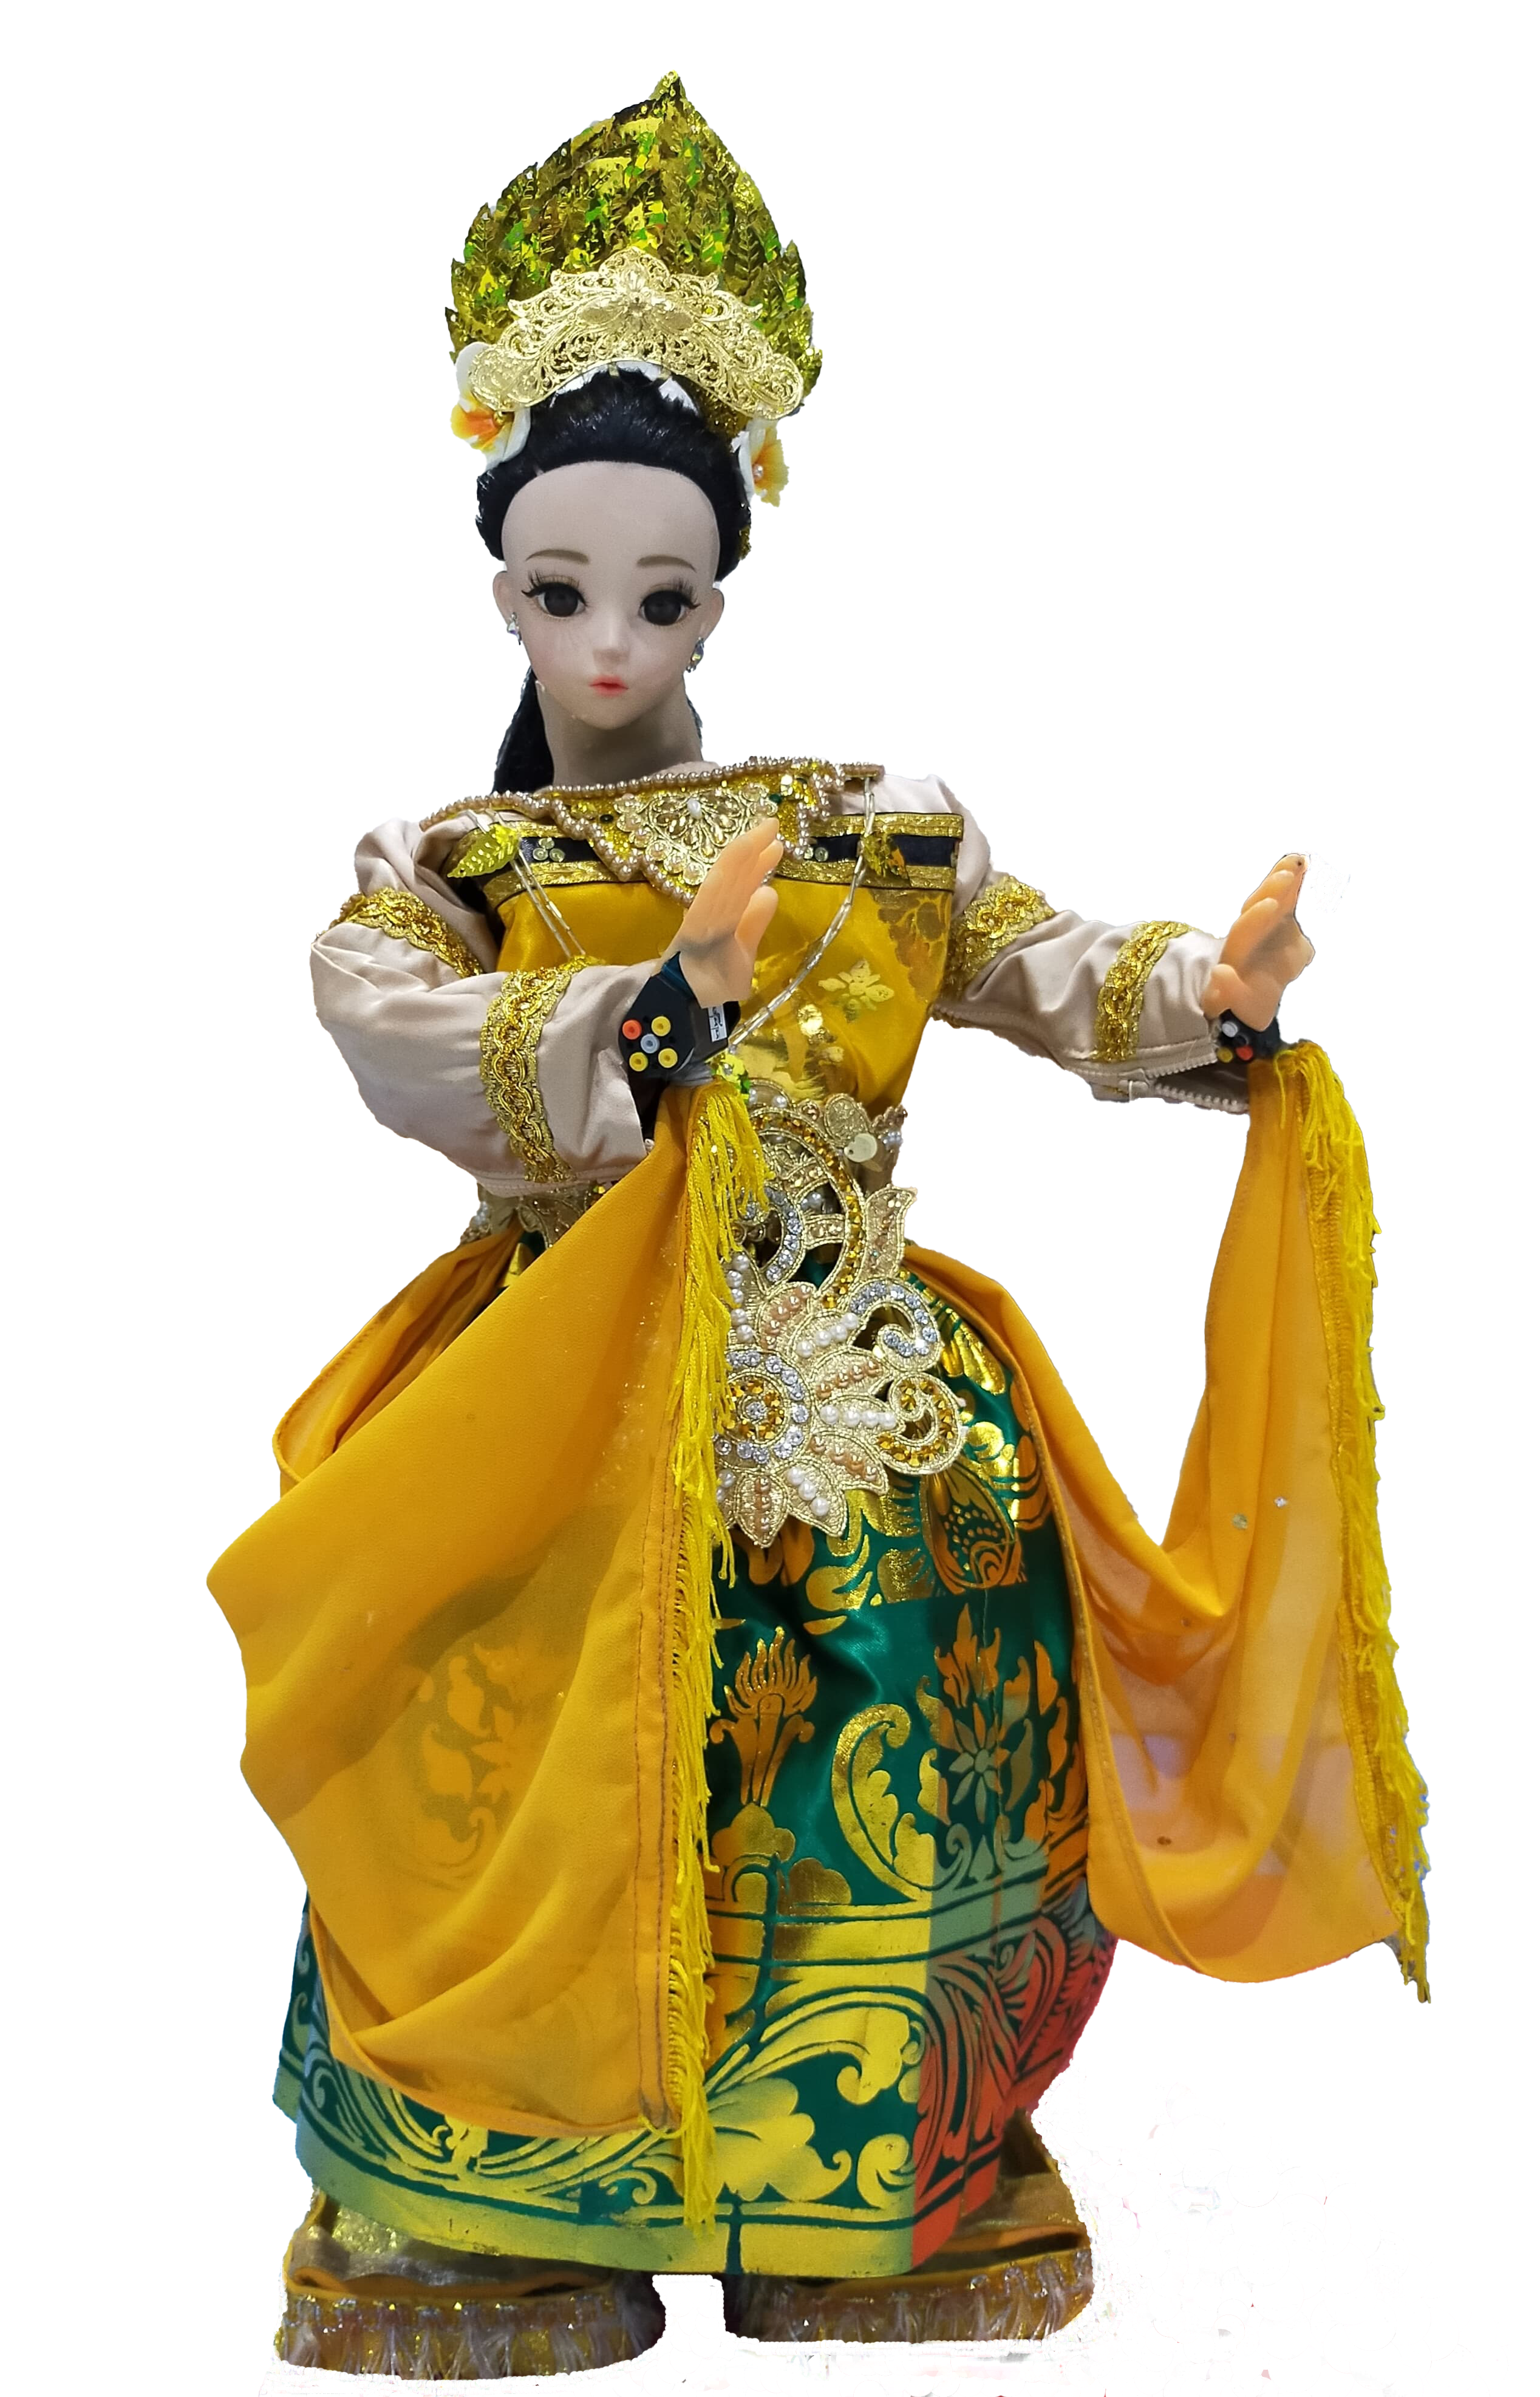
\includegraphics[width=\textwidth]{./images/actual_robot.png}
		\caption{}
		\label{fig:actual_robot}
	\end{subfigure}
	\caption{The Barelang 7 humanoid robot: (a) Mechanical design, and (b) Actual physical robot.}
	\label{fig:robot_all}
\end{figure}

\subsection{Proposed speech-based question-answering system}
Fig. \ref{fig:qa} depicts the proposed question-answering (QA) system. The procedure commences by acquiring speech signals as auditory data from a microphone. The audio data is subsequently transformed into byte format and subjected to VOSK processing to transcribe the speech into text automatically. The transcribed text constitutes the input for the QA procedure. Furthermore, contextual information is included to assist the algorithm in locating pertinent replies to the given inquiry.

Subsequently, the question and context are prepared for analysis by the QA model, which computes a logit to forecast the initial and final positions of the response within the given context. The model identifies tokens that are most likely indicative of the start and conclusion of the response. Subsequently, these tokens are isolated from the surrounding context and converted into a comprehensible textual structure, subsequently provided as the ultimate response.

Furthermore, the system employs text-to-speech (TTS) technology to transform the answer provided in text format into audible speech. The TTS process entails the analysis of text to comprehend the pronunciation of individual words, converting text into phonemes, and generating sound waves based on these selected phonemes. Upon collection in an audio buffer, the sound waves undergo processing to provide the ultimate spoken output.

\begin{figure}[t]
	\centering
	\includegraphics[width=1\textwidth]{./images/qa-new.png}
	\caption{Block diagram of the speech-based question-answering system.}
	\label{fig:qa}
\end{figure}

\subsection{Implementation of automatic speech recognition}
Automatic speech recognition (ASR) is the technology that automates the conversion of human speech into a written format suitable for computer processing. As illustrated in Fig \ref{fig:asr}, the ASR procedure starts by recording human speech as an audio signal represented as a waveform. This audio stream is subjected to multiple processing stages, including filtering to eliminate noise and feature extraction to detect important speech attributes. Furthermore, the ASR system examines these characteristics to generate a textual result corresponding to spoken words. One essential component of ASR is phoneme processing, which involves decomposing speech into its smallest sound components, known as phonemes, to differentiate between words. As an illustration, the word ``tree" can be deconstructed phonetically into the individual sounds /t/ - /r/ - /i/.

\begin{figure}[t]
	\centering
	\includegraphics[width=1\textwidth]{./images/asr.png}
	\caption{Block diagram of the automatic speech recognition (ASR).}
	\label{fig:asr}
\end{figure}

This work utilized VOSK, a freely available ASR toolbox, as the paradigm for speech recognition. VOSK, which has been actively developed since 2019, provides a wide range of features and facilitates offline voice recognition. The existing API version, 0.3.45, utilizes advanced deep learning algorithms to detect distinct patterns in sound and precisely convert spoken words into written text. The selection of VOSK was motivated by its strength in effectively processing different accents and languages, rendering it an appropriate model for our specific application.

\subsection{Implementation of the RoBERTa model}
The Robustly Optimized BERT Pre-training Approach (RoBERTa) is an advanced natural language processing (NLP) model, serving as a modified version of the widely used Bidirectional Encoder Representations from Transformers (BERT) model. RoBERTa undergoes training on an extensive collection of self supervised English text data. During training, 15\% of the words in each input sentence are randomly concealed. The model is required to accurately predict these concealed words to acquire language patterns most efficiently. By employing this method, RoBERTa can acquire a profound comprehension of context and semantics, rendering it especially suitable for tasks involving answering questions.

The present research employs RoBERTa as the fundamental element of the (QA) system. Using its sophisticated language comprehension abilities, the model analyzes the input text obtained by ASR and produces precise answers to the given questions. The selection of RoBERTa was motivated by its exceptional performance in specific NLP tasks, such as question answering, where it has repeatedly shown cutting edge outcomes.

Fig \ref{fig:gui} illustrates the architecture of a graphical user interface (GUI) intended to identify speech, compute the word error rate (WER), determine the reaction time, and deliver responses to the provided queries. The graphical user interface (GUI) system was developed using the Python programming language and Tkinter, as suggested by \cite{Venkata_Naga_Nymisha2024-uw}. In this system, voice recognition will occur after activating the start button. Upon speech recognition, the system will produce the query's WER and the temporal response time needed to generate the answer.

\begin{figure}[t]
	\centering
	\includegraphics[width=1\textwidth]{./images/gui.png}
	\caption{Graphical User Interface (GUI) of the question-answering system.}
	\label{fig:gui}
\end{figure}

\subsection{Implementation of text-to-speech}
Text-to-speech (TTS) is a technology that transforms textual input into audible voice, facilitating human-computer interaction by vocal communication. The present work employed the pyttsx3 library in Python, which presents notable benefits compared to alternative TTS libraries. A key advantage of this technology is its offline capability, which enhances its reliability in settings with unpredictable internet connectivity. Unlike specific TTS libraries that require saving text as an audio file before playback, pyttsx3 can rapidly generate and play the speech output in real-time. This feature significantly improves the user experience by minimizing latency. In addition, pyttsx3 enables the customization of the voice output, encompassing modifications to volume, pitch, and gender, therefore allowing for the adaptation to suit particular user preferences. The selection of pyttsx3 was motivated by its interoperability with the broader Python ecosystem and its versatility in different application scenarios, especially in robotics, where dynamic and flexible speech output is crucial.

\section{Result and discussion}
The following part provides and analyzes the findings derived from the study, starting with a description of the assessment techniques used. A comprehensive account of the data gathering procedure is also provided to verify the research results. The following subsections (3.1 and 3.2) comprehensively examine the experimental findings, with a specific emphasis on essential performance indicators and their consequences for the suggested system.

\subsection{Evaluation methods}
The evaluation of proposed speech-based question-answering (QA) system primarily included the assessment of two critical performance metrics: word error rate (WER) and response time. These metrics are essential for evaluating the efficacy and efficiency of the system in practical applications.

The word error rate (WER) is widely used for assessing automatic speech recognition (ASR) systems. This metric quantifies the precision of transcribed text concerning the source text. The formula for computing WER is given by Equation \ref{eq:wer}.

\begin{equation}
	WER = \frac{S+D+I}{N}
	\label{eq:wer}
\end{equation}

The variable $S$ denotes the number of substitutions, $D$ represents the number of deletions, $I$ represents the number of insertions, and $N$ represents the total amount of words in the reference text. A reduced WER shows greater accuracy in the ASR system. In order to evaluate the system's ability to handle different accents and pronunciations, this work computed the WER using tests performed with non-native English speakers.

Response time is a crucial factor in assessing the effectiveness of a question-answering system, especially in applications that require immediate response. The response time is the duration between original speech input and the system's production of the matching response, which is mathematically represented by Equation \ref{eq:dt}. Symbol $t_0$ represents the initiation of voice input processing by the system, while $t$ is the moment when response is produced. Efficient systems are characterized by quicker response time, enhancing the user experience.

\begin{equation}
	\delta{t}=t-t_0
	\label{eq:dt}
\end{equation}

The results obtained from the WER and response time evaluations offer valuable insights into the broad performance of the speech-based question-answering system. These results reveal both areas of proficiency and opportunities for enhancement.

\subsection{Evaluation results}
The present experiment evaluated the system using a microphone to record spoken signals in real-time. The system produced replies to a predetermined series of inquiries posed to the robot, including ``Where is the immigration office?", ``Where is the mayor's office?", ``Where is the airport?", ``Where is the nearest gas station?" and ``Where is the nearest hospital?". The system performed testing with a sample of five distinct speakers, three Indonesian person, and two French males, to verify accuracy of the findings. Each speaker in the study posed five questions 5 times, totaling 125 trials.

The trial resulted in a WER of 0.187, demonstrating the system's precision in transcribing spoken language into written text. In particular, the experiment documented 86 instances of word replacements, 5 instances of word deletions, and 22 instances of word insertions. The inaccuracies detected in the predictions of ASR system are elaborated on in Table \ref{tab:common_errors}. For instance, the question ``Where is the nearest gas station?" had the highest error rate, with the ASR system frequently misinterpreting ``gas station" as ``guess", ``news", ``when", or ``new has". Similarly, ``Where is the mayor's office?" was often misrecognized, with the ASR producing variations such as ``manager's", ``your main" and ``his meal movies". A notable error occurred with the question ``Where is the airport?" spoken by FR1, where it was incorrectly transcribed as ``Where is the half pot?"—though this error occurred only once during the trials.

\begin{table}[t]
	\caption{Common errors in ASR predictions.}
	\label{tab:common_errors} 
	\begin{center}
		\begin{tabular}{r@{\quad}ll}
			\hline
			\multicolumn{1}{l}{\rule{0pt}{12pt} Person} & \multicolumn{1}{l}{Spoken question} & \multicolumn{1}{l}{Recognized question} \\[2pt]
			\hline\rule{0pt}{12pt}
			ID1 & Where is the mayor's office? & Where is the manager's office? \\
			ID2 & Where is the mayor's office? & Where is the main your office? \\
			ID2 & Where is the nearest gas station? & Where is the nearest guess the shin? \\
			ID3 & Where is the nearest gas station? & Where is the news gas station? \\
			FR1 & Where is the nearest gas station? & When is the nearest gas station? \\
			FR1 & Where is the airport? & Where is of half pot? \\
			FR1 & Where is the nearest hospital? & Where is the newest was beaten? \\
			FR2 & Where is the mayor's office? & Where his meal movies? \\[2pt]
			\hline
		\end{tabular}
	\end{center}
\end{table}

\begin{table}[t]
	\caption{Response times for QA system across different spoken questions.}
	\label{tab:response_time} 
	\begin{center}
		\begin{tabular}{r@{\quad}r@{\quad}l@{\quad}rrr}
			\hline
			\multicolumn{1}{l}{\rule{0pt}{12pt} No} & \multicolumn{1}{l}{Person} & \multicolumn{1}{l}{Spoken question} & \multicolumn{1}{l}{Fastest (ms)} & \multicolumn{1}{l}{Slowest (ms)} & \multicolumn{1}{l}{Average (ms)} \\[2pt]
			\hline\rule{0pt}{12pt}
			1 & ID1 & Where is the immigration office? & 430 & 720 & 550 \\
			2 & ID1 & Where is the mayor's office? & 510 & 1640 & 794 \\
			3 & ID1 & Where is the airport? & 480 & 650 & 590 \\
			4 & ID1 & Where is the nearest gas station? & 510 & 760 & 616 \\
			5 & ID1 & Where is the nearest hospital? & 490 & 650 & 556 \\
			6 & ID2 & Where is the immigration office? & 550 & 700 & 634 \\
			7 & ID2 & Where is the mayor's office? & 490 & 770 & 584 \\
			8 & ID2 & Where is the airport? & 440 & 510 & 484 \\
			9 & ID2 & Where is the nearest gas station? & 530 & 630 & 578 \\
			10 & ID2 & Where is the nearest hospital? & 500 & 580 & 548 \\
			11 & ID3 & Where is the immigration office? & 260 & 350 & 298 \\
			12 & ID3 & Where is the mayor's office? & 250 & 310 & 278 \\
			13 & ID3 & Where is the airport? & 230 & 310 & 268 \\
			14 & ID3 & Where is the nearest gas station? & 270 & 390 & 318 \\
			15 & ID3 & Where is the nearest hospital? & 280 & 350 & 312 \\
			16 & FR1 & Where is the immigration office? & 330 & 1060 & 536 \\
			17 & FR1 & Where is the mayor's office? & 320 & 530 & 394 \\
			18 & FR1 & Where is the airport? & 340 & 430 & 370 \\
			19 & FR1 & Where is the nearest gas station? & 290 & 490 & 356 \\
			20 & FR1 & Where is the nearest hospital? & 350 & 490 & 418 \\
			21 & FR2 & Where is the immigration office? & 300 & 540 & 368 \\
			22 & FR2 & Where is the mayor's office? & 330 & 470 & 400 \\
			23 & FR2 & Where is the airport? & 360 & 610 & 430 \\
			24 & FR2 & Where is the nearest gas station? & 310 & 600 & 438 \\
			25 & FR2 & Where is the nearest hospital? & 410 & 530 & 458 \\[2pt]
			\hline
		\end{tabular}
	\end{center}
\end{table}

After conducting 125 tests, the mean system response time was 464.04 milliseconds. The system's response time during testing, derived from 125 trials, is presented in Table \ref{tab:response_time}. The system had quickest response time in this test when speakers ID3 spoke to the robot. Tested with ID3 speaker, the shortest reaction time recorded was 390 milliseconds. Meanwhile, the system exhibited slowest reaction time when an ID1 was spoken during the test.

\section{Conclusion and future work}
This paper describes developing and evaluating a speech-automated question-answering system using the Barelang 7 humanoid robot platform. The proposed system employed VOSK for automatic speech recognition (ASR), RoBERTa for question answering, and pyttsx3 for text-to-speech (TTS). The assessment centered on two primary performance indicators: word error rate (WER) and response time.

The results indicated that the system attained a WER of 0.187 across 125 trials, with the most significant error rates recorded in queries that included less frequently used terms or intricate sentences. The mean response time was 464.04 milliseconds, exhibiting fluctuations according to the speaker and intricacy of the question. Investigation emphasized the system's capacity to manage various accents and pronunciations. However, additional ASR accuracy and response time enhancements are required to improve the overall user experience significantly.

In summary, the research has effectively showcased the capacity of combining ASR, QA, and TTS technologies into a unified system on a humanoid robot platform. Nevertheless, it is imperative for future research to prioritize the enhancement of ASR model in order to minimize mistake rates, optimize the system's capacity to comprehend and react to a broader array of accents and languages, and optimize the response time for real-time applications.

\section*{Acknowledgement}
This research is one of the project-based learning outcome and the student's final project in the Department of Electrical Engineering, Politeknik Negeri Batam. We thank the Politeknik Negeri Batam and BRAIL for facilitating and providing equipment to support the research.

%
% ---- Bibliography ----
%
\begin{thebibliography}{9}
	
	\bibitem{Roda-Sanchez2021-rm}Roda-Sanchez, L., Olivares, T., Garrido-Hidalgo, C., Vara, J. \& Fernández-Caballero, A. Human-robot interaction in Industry 4.0 based on an Internet of Things real-time gesture control system. {\em Integr. Comput. Aided Eng.}. \textbf{28}, 159-175 (2021,3), doi: 10.3233/ICA-200637.
	
	\bibitem{Angleraud2021-lp}Angleraud, A., Mehman Sefat, A., Netzev, M. \& Pieters, R. Coordinating shared tasks in human-robot collaboration by commands. {\em Front. Robot. AI}. \textbf{8} (2021,10), doi: 10.3389/frobt.2021.734548.
	
	\bibitem{Mawaddah2024-ii}Mawaddah, N., Tamba, C., Hutagalung, D., Nainggolan, F., Lubis, E. \& Jamzuri, E. Automatic speech recognition for human-robot interaction on the humanoid robot barelang 7. {\em Proceedings Of The 6th International Conference On Applied Engineering, ICAE 2023, 7 November 2023, Batam, Riau Islands, Indonesia}. (2024), doi: 10.4108/eai.7-11-2023.2342940.
	
	\bibitem{Unlu2019-xa}Unlu, M., Arisoy, E. \& Saraclar, M. Question answering for spoken lecture processing. {\em ICASSP 2019 - 2019 IEEE International Conference On Acoustics, Speech And Signal Processing (ICASSP)}. \textbf{abs 1608 7905} pp. 7365-7369 (2019,5), doi: 10.1109/ICASSP.2019.8682580.

	\bibitem{Yossy2021-pq}Yossy, E. \& Hana, W. Knowledge-based chatbot for humanoid robot in restaurant for question and answering system. {\em ICIC Express Letters, Part B: Applications}. \textbf{13}, 315-320 (2021), doi: 10.24507/icicelb.13.03.315.
		
	\bibitem{Abubakar2020-ha}Abubakar, S., Das, S., Robinson, C., Saadatzi, M., Logsdon, M., Mitchell, H., Chlebowy, D. \& Popa, D. ARNA, a service robot for nursing assistance: System overview and user acceptability. {\em 2020 IEEE 16th International Conference On Automation Science And Engineering (CASE)}. (2020,8), doi: 10.1109/CASE48305.2020.9216845.
		
	\bibitem{Berezina2019-mk}Berezina, K., Ciftci, O. \& Cobanoglu, C. Robots, Artificial Intelligence, and Service Automation in Restaurants. {\em Robots, Artificial Intelligence, And Service Automation In Travel, Tourism And Hospitality}. pp. 185-219 (2019,10), doi: 10.1108/978-1-78756-687-320191010.
	
	\bibitem{Fukumori2022-ni}Fukumori, T., Cai, C., Zhang, Y., El Hafi, L., Hagiwara, Y., Nishiura, T. \& Taniguchi, T. Optical laser microphone for human-robot interaction: speech recognition in extremely noisy service environments. {\em Adv. Robot.}. \textbf{36}, 304-317 (2022,3), doi: 10.1080/01691864.2021.2023629.
	
	\bibitem{Venkata_Naga_Nymisha2024-uw}Venkata Naga Nymisha, T., Pavan Kumar, C., Abhi Venkata Sai, S. \& Mounica Kaumudhi, B. A deep learning-based face recognition model for comprehensive student logging mechanism using tkinter. {\em Lecture Notes In Electrical Engineering}. pp. 239-248 (2024), doi: 10.1007/978-981-97-0644-0\_22.
	
\end{thebibliography}

\end{document}
